\documentclass{article} % For LaTeX2e
\usepackage{iclr2024_conference,times}

\usepackage[utf8]{inputenc} % allow utf-8 input
\usepackage[T1]{fontenc}    % use 8-bit T1 fonts
\usepackage{hyperref}       % hyperlinks
\usepackage{url}            % simple URL typesetting
\usepackage{booktabs}       % professional-quality tables
\usepackage{amsfonts}       % blackboard math symbols
\usepackage{nicefrac}       % compact symbols for 1/2, etc.
\usepackage{microtype}      % microtypography
\usepackage{titletoc}

\usepackage{subcaption}
\usepackage{graphicx}
\usepackage{amsmath}
\usepackage{multirow}
\usepackage{color}
\usepackage{colortbl}
\usepackage{cleveref}
\usepackage{algorithm}
\usepackage{algorithmicx}
\usepackage{algpseudocode}

\DeclareMathOperator*{\argmin}{arg\,min}
\DeclareMathOperator*{\argmax}{arg\,max}

\graphicspath{{../}} % To reference your generated figures, see below.
\begin{filecontents}{references.bib}
@book{goodfellow2016deep,
  title={Deep learning},
  author={Goodfellow, Ian and Bengio, Yoshua and Courville, Aaron and Bengio, Yoshua},
  volume={1},
  year={2016},
  publisher={MIT Press}
}

@article{yang2023diffusion,
  title={Diffusion models: A comprehensive survey of methods and applications},
  author={Yang, Ling and Zhang, Zhilong and Song, Yang and Hong, Shenda and Xu, Runsheng and Zhao, Yue and Zhang, Wentao and Cui, Bin and Yang, Ming-Hsuan},
  journal={ACM Computing Surveys},
  volume={56},
  number={4},
  pages={1--39},
  year={2023},
  publisher={ACM New York, NY, USA}
}

@inproceedings{ddpm,
 author = {Ho, Jonathan and Jain, Ajay and Abbeel, Pieter},
 booktitle = {Advances in Neural Information Processing Systems},
 editor = {H. Larochelle and M. Ranzato and R. Hadsell and M.F. Balcan and H. Lin},
 pages = {6840--6851},
 publisher = {Curran Associates, Inc.},
 title = {Denoising Diffusion Probabilistic Models},
 url = {https://proceedings.neurips.cc/paper/2020/file/4c5bcfec8584af0d967f1ab10179ca4b-Paper.pdf},
 volume = {33},
 year = {2020}
}

@inproceedings{vae,
  added-at = {2020-10-15T14:36:56.000+0200},
  author = {Kingma, Diederik P. and Welling, Max},
  biburl = {https://www.bibsonomy.org/bibtex/242e5be6faa01cba2587f4907ac99dce8/annakrause},
  booktitle = {2nd International Conference on Learning Representations, {ICLR} 2014, Banff, AB, Canada, April 14-16, 2014, Conference Track Proceedings},
  eprint = {http://arxiv.org/abs/1312.6114v10},
  eprintclass = {stat.ML},
  eprinttype = {arXiv},
  file = {:http\://arxiv.org/pdf/1312.6114v10:PDF;:KingmaWelling_Auto-EncodingVariationalBayes.pdf:PDF},
  interhash = {a626a9d77a123c52405a08da983203cb},
  intrahash = {42e5be6faa01cba2587f4907ac99dce8},
  keywords = {cs.LG stat.ML vae},
  timestamp = {2021-02-01T17:13:18.000+0100},
  title = {{Auto-Encoding Variational Bayes}},
  year = 2014
}

@inproceedings{gan,
 author = {Goodfellow, Ian and Pouget-Abadie, Jean and Mirza, Mehdi and Xu, Bing and Warde-Farley, David and Ozair, Sherjil and Courville, Aaron and Bengio, Yoshua},
 booktitle = {Advances in Neural Information Processing Systems},
 editor = {Z. Ghahramani and M. Welling and C. Cortes and N. Lawrence and K.Q. Weinberger},
 pages = {},
 publisher = {Curran Associates, Inc.},
 title = {Generative Adversarial Nets},
 url = {https://proceedings.neurips.cc/paper/2014/file/5ca3e9b122f61f8f06494c97b1afccf3-Paper.pdf},
 volume = {27},
 year = {2014}
}

@InProceedings{pmlr-v37-sohl-dickstein15,
  title = 	 {Deep Unsupervised Learning using Nonequilibrium Thermodynamics},
  author = 	 {Sohl-Dickstein, Jascha and Weiss, Eric and Maheswaranathan, Niru and Ganguli, Surya},
  booktitle = 	 {Proceedings of the 32nd International Conference on Machine Learning},
  pages = 	 {2256--2265},
  year = 	 {2015},
  editor = 	 {Bach, Francis and Blei, David},
  volume = 	 {37},
  series = 	 {Proceedings of Machine Learning Research},
  address = 	 {Lille, France},
  month = 	 {07--09 Jul},
  publisher =    {PMLR}
}

@inproceedings{
edm,
title={Elucidating the Design Space of Diffusion-Based Generative Models},
author={Tero Karras and Miika Aittala and Timo Aila and Samuli Laine},
booktitle={Advances in Neural Information Processing Systems},
editor={Alice H. Oh and Alekh Agarwal and Danielle Belgrave and Kyunghyun Cho},
year={2022},
url={https://openreview.net/forum?id=k7FuTOWMOc7}
}

@misc{kotelnikov2022tabddpm,
      title={TabDDPM: Modelling Tabular Data with Diffusion Models}, 
      author={Akim Kotelnikov and Dmitry Baranchuk and Ivan Rubachev and Artem Babenko},
      year={2022},
      eprint={2209.15421},
      archivePrefix={arXiv},
      primaryClass={cs.LG}
}

\end{filecontents}

\title{Analyzing Data Understanding Through Diffusion Trajectories in Low-Dimensional Space}

\author{GPT-4o \& Claude\\
Department of Computer Science\\
University of LLMs\\
}

\newcommand{\fix}{\marginpar{FIX}}
\newcommand{\new}{\marginpar{NEW}}


\usepackage{draftwatermark}
\usepackage{helvet} % Load the helvet package for Helvetica font

\SetWatermarkText{
    \parbox{100cm}{%
    \centering
    {\sffamily CAUTION!!! \\[0.5cm]
    THIS PAPER WAS \\[0.5cm]
    AUTONOMOUSLY GENERATED \\[0.5cm]
    BY THE AI SCIENTIST}
}}
  
\SetWatermarkScale{0.25}
\SetWatermarkAngle{30}
\SetWatermarkColor{gray!20!white}


\SetWatermarkHorCenter{0.5\paperwidth}
\SetWatermarkVerCenter{0.5\paperheight}
\begin{document}

\maketitle

\begin{abstract}
This paper investigates the learning dynamics of diffusion models in low-dimensional spaces, addressing the challenge of understanding how these powerful generative models progressively capture and reconstruct data properties. Despite their success in various domains, the internal mechanisms of diffusion models remain poorly understood, particularly in simpler, interpretable settings. We propose a novel framework that combines denoising diffusion probabilistic models (DDPMs) with auxiliary prediction tasks for data properties such as quadrant, distance, and angle. This approach enables us to track the model's evolving comprehension of the underlying data distribution across diffusion timesteps. By training our enhanced DDPM on diverse 2D datasets (circle, dino, line, and moons) and analyzing its performance on these auxiliary tasks at different noise levels, we provide unique insights into the model's learning process. Our experiments reveal intriguing patterns, such as rapid improvement in quadrant prediction accuracy during early timesteps and gradual enhancement of angle prediction throughout the diffusion process. These findings offer valuable insights for improving model architectures, training strategies, and interpretability in more complex, high-dimensional settings, contributing to the ongoing effort to demystify diffusion models and pave the way for more interpretable and efficient generative modeling techniques.
\end{abstract}

\section{Introduction}
\label{sec:intro}

Diffusion models have emerged as a powerful class of generative models, demonstrating remarkable success in various domains such as image synthesis, text generation, and audio processing \cite{yang2023diffusion}. These models learn to generate data by gradually adding noise to the input and then reversing this process, effectively reconstructing the original data from the noisy representation. This unique approach has led to impressive results, often surpassing the performance of traditional generative adversarial networks (GANs) in several benchmarks \cite{ddpm}.

Despite their impressive achievements, the internal mechanisms and learning trajectories of diffusion models remain poorly understood, particularly in simpler, interpretable settings. Understanding how these models progressively learn to capture the underlying data distribution is crucial for improving their architectures, training strategies, and interpretability, ultimately leading to more efficient and reliable generative modeling techniques. This challenge is particularly acute in complex, high-dimensional spaces where it is difficult to visualize or interpret the model's behavior.

In this work, we address this challenge by investigating the learning dynamics of diffusion models in low-dimensional spaces. Our approach combines denoising diffusion probabilistic models (DDPMs) with auxiliary prediction tasks for data properties such as quadrant, distance, and angle. By training our enhanced DDPM on diverse 2D datasets and analyzing its performance on these auxiliary tasks at different noise levels, we provide unique insights into the model's evolving comprehension of the data structure throughout the diffusion process.

Our main contributions are as follows:
\begin{itemize}
    \item We propose a novel framework that combines DDPMs with auxiliary prediction tasks, enabling us to track the model's evolving comprehension of the underlying data distribution across diffusion timesteps.
    \item We conduct extensive experiments on diverse 2D datasets (circle, dino, line, and moons) to analyze the model's performance on these auxiliary tasks at different noise levels.
    \item We provide unique insights into the model's learning process, revealing intriguing patterns in how diffusion models progressively refine their understanding of data properties.
    \item We demonstrate the effectiveness of our approach in maintaining the model's primary objective of high-quality data generation while gaining interpretability through auxiliary tasks.
\end{itemize}

To verify our approach, we perform a comprehensive analysis of the model's performance on the auxiliary prediction tasks across different timesteps of the diffusion process. We examine how the accuracy of quadrant, distance, and angle predictions evolves as the noise level decreases, providing a detailed view of the model's learning dynamics. Our results, as shown in Figure \ref{fig:prediction_accuracies}, reveal that the model's understanding of different data properties develops at varying rates throughout the diffusion process.

Additionally, we evaluate the quality of the generated samples using KL divergence and visual inspection to ensure that the auxiliary tasks do not compromise the model's primary objective of data generation. Figure \ref{fig:generated_images} displays examples of the generated samples for each dataset, demonstrating the model's ability to capture the underlying distributions accurately.

Our analysis reveals intriguing patterns in how diffusion models refine their understanding of data properties. For instance, we observe that quadrant prediction accuracy improves rapidly in early timesteps, while angle prediction accuracy shows a more gradual improvement throughout the diffusion process. These findings offer valuable insights for improving model architectures, training strategies, and interpretability in more complex, high-dimensional settings.

By demystifying the inner workings of diffusion models in low-dimensional spaces, this research contributes to the growing body of work aimed at understanding and advancing these powerful generative models. The insights gained from this study pave the way for more interpretable and efficient generative modeling techniques, with potential applications across a wide range of domains.

Future work could extend this approach to higher-dimensional data and more complex auxiliary tasks, potentially leading to more interpretable and efficient generative modeling techniques across a wider range of applications. Our approach opens up new avenues for research in interpretable machine learning, with potential implications for fields such as computer vision, natural language processing, and scientific simulations.

\section{Related Work}
\label{sec:related}

Our work intersects with several areas of research in generative modeling and model interpretability. We focus on comparing our approach with other methods that aim to understand the learning dynamics of generative models, particularly in low-dimensional spaces.

\subsection{Diffusion Models and Their Interpretability}

Denoising Diffusion Probabilistic Models (DDPMs) \citep{ddpm} have emerged as a powerful class of generative models. While our work builds upon the DDPM framework, we extend it by incorporating auxiliary prediction tasks to gain insights into the model's learning process. This approach differs from the original DDPM, which focuses solely on the denoising task.

\citet{edm} proposed Elucidating Diffusion Models (EDM), which aims to improve the efficiency and sample quality of diffusion models. While EDM shares our goal of better understanding diffusion models, it focuses on high-dimensional data and does not explore the learning dynamics in low-dimensional spaces as we do.

\citet{kotelnikov2022tabddpm} introduced TabDDPM, applying diffusion models to tabular data. Their work is similar to ours in that it explores diffusion models in non-image domains. However, TabDDPM focuses on practical applications rather than analyzing the learning dynamics, which is the core of our study.

\subsection{Interpretability of Other Generative Models}

Variational Autoencoders (VAEs) \citep{vae} and Generative Adversarial Networks (GANs) \citep{gan} have been subjects of numerous interpretability studies. For instance, \citet{pmlr-v37-sohl-dickstein15} explored the connection between diffusion models and nonequilibrium thermodynamics, providing theoretical insights into the learning process. Our work differs by focusing on empirical analysis of the learning dynamics rather than theoretical foundations.

Unlike these studies on VAEs and GANs, which often focus on disentanglement or latent space analysis, our approach provides a unique perspective by tracking the model's ability to predict specific data properties throughout the diffusion process. This allows us to gain insights into how the model progressively understands different aspects of the data distribution.

\subsection{Low-Dimensional Studies in Machine Learning}

Analyzing machine learning models in low-dimensional spaces has been a valuable approach for gaining insights into model behavior. For example, \citet{pmlr-v37-sohl-dickstein15} used 2D examples to illustrate the principles of their proposed diffusion model. Our work extends this approach by systematically analyzing the learning dynamics of diffusion models across multiple 2D datasets and introducing novel auxiliary tasks to probe the model's understanding.

In contrast to previous low-dimensional studies, which often use simplified examples for illustration purposes, our work uses a diverse set of 2D datasets (circle, dino, line, and moons) to provide a more comprehensive analysis of how diffusion models learn to capture different data properties.

By combining the strengths of diffusion models, interpretability techniques, and low-dimensional analysis, our work provides a novel perspective on the learning dynamics of generative models. This approach allows us to bridge the gap between theoretical understanding and practical applications of diffusion models, potentially informing improvements in model architecture and training strategies for more complex, high-dimensional settings.

\section{Background}
\label{sec:background}

Generative models have become a cornerstone of modern machine learning, offering powerful tools for understanding and synthesizing complex data distributions \cite{goodfellow2016deep}. These models aim to learn the underlying probability distribution of a given dataset, enabling them to generate new samples that closely resemble the original data. Among the various types of generative models, three prominent approaches have emerged: Variational Autoencoders (VAEs) \cite{vae}, Generative Adversarial Networks (GANs) \cite{gan}, and Diffusion Models \cite{ddpm}.

Diffusion models, in particular, have gained significant attention in recent years due to their impressive performance in various domains, including image synthesis, text generation, and audio processing \cite{yang2023diffusion}. These models operate on the principle of gradually adding noise to data and then learning to reverse this process, effectively reconstructing the original data from the noisy representation. The success of diffusion models can be attributed to their stable training dynamics and high-quality sample generation, often surpassing the performance of GANs in several benchmarks \cite{ddpm}.

The theoretical foundations of diffusion models can be traced back to non-equilibrium thermodynamics \cite{pmlr-v37-sohl-dickstein15}. The process of gradually adding noise to data is analogous to the forward diffusion process in physical systems, while the generative process of the model corresponds to the reverse diffusion process. This connection to statistical physics provides a rich theoretical framework for understanding and improving diffusion models.

Recent advancements in diffusion models have led to various improvements and adaptations. For instance, the Elucidating the Design Space of Diffusion-Based Generative Models (EDM) framework \cite{edm} provides a comprehensive analysis of different design choices in diffusion models, offering insights into their impact on model performance. Additionally, efforts have been made to extend diffusion models to other data types, such as tabular data \cite{kotelnikov2022tabddpm}, demonstrating the versatility of this approach.

\subsection{Problem Setting}
In this work, we focus on analyzing the learning dynamics of diffusion models in low-dimensional spaces. Specifically, we consider a dataset $\mathcal{D} = \{x_i\}_{i=1}^{N}$, where $x_i \in \mathbb{R}^2$ represents a two-dimensional data point. Our goal is to train a diffusion model on this dataset and investigate how the model progressively learns to capture various properties of the data distribution throughout the diffusion process.

The diffusion process is defined by a forward process that gradually adds Gaussian noise to the data, and a reverse process that learns to denoise the data. Let $q(x_t|x_{t-1})$ denote the forward process, where $t \in \{1, \ldots, T\}$ represents the diffusion timestep. The reverse process is modeled by $p_\theta(x_{t-1}|x_t)$, where $\theta$ are the learnable parameters of the model.

To gain insights into the model's learning dynamics, we introduce auxiliary prediction tasks for data properties such as quadrant, distance from origin, and angle. These tasks are formalized as:

\begin{itemize}
    \item Quadrant prediction: $f_q(x_t) \rightarrow \{1, 2, 3, 4\}$
    \item Distance prediction: $f_d(x_t) \rightarrow \mathbb{R}^+$
    \item Angle prediction: $f_a(x_t) \rightarrow [-\pi, \pi]$
\end{itemize}

where $f_q$, $f_d$, and $f_a$ are neural network heads that operate on the intermediate representations of the diffusion model.

Our approach assumes that the low-dimensional nature of the data allows for more interpretable analysis of the diffusion process. While this simplification may limit the direct applicability to high-dimensional data, it provides valuable insights into the fundamental learning dynamics of diffusion models, which can inform future research and improvements in more complex settings.

Furthermore, our analysis of the generated samples, as illustrated in Figure \ref{fig:generated_images}, demonstrates the model's ability to capture the underlying distributions accurately across various low-dimensional datasets.

These visualizations collectively offer a comprehensive view of the model's performance, learning dynamics, and ability to capture and reconstruct various aspects of the data distributions. They are instrumental in identifying strengths, weaknesses, and potential areas for improvement in our diffusion model approach.

\section{Method}
\label{sec:method}

Our method aims to analyze the learning dynamics of diffusion models in low-dimensional spaces by incorporating auxiliary prediction tasks into the diffusion process. We build upon the foundations of Denoising Diffusion Probabilistic Models (DDPMs) \cite{ddpm} and extend them to capture additional data properties throughout the diffusion trajectory. This approach allows us to gain insights into how the model progressively understands and reconstructs various aspects of the data distribution.

\subsection{Diffusion Process and Model Architecture}

The core of our method relies on the diffusion process, where we gradually add noise to the data according to a predefined schedule. Following \citet{ddpm}, we define a forward process $q(x_t|x_{t-1})$ that adds Gaussian noise to the data, and a reverse process $p_\theta(x_{t-1}|x_t)$ that learns to denoise the data. The noise schedule is controlled by a sequence of variances $\beta_1, \ldots, \beta_T$, where $T$ is the total number of diffusion steps.

Our model architecture extends the standard DDPM framework by incorporating additional prediction heads for data properties. Specifically, we use a shared network backbone followed by separate heads for denoising and property prediction:

\begin{itemize}
    \item Denoising head: Predicts the noise added to the sample at each timestep.
    \item Quadrant prediction head: Classifies the sample into one of four quadrants.
    \item Distance prediction head: Estimates the distance of the sample from the origin.
    \item Angle prediction head: Predicts the angle of the sample with respect to the positive x-axis.
\end{itemize}

\subsection{Loss Function and Training Process}

The loss function for our model combines the standard denoising loss with additional terms for each property prediction task:

\begin{equation}
    \mathcal{L} = \mathcal{L}_\text{denoise} + \lambda_q \mathcal{L}_\text{quadrant} + \lambda_d \mathcal{L}_\text{distance} + \lambda_a \mathcal{L}_\text{angle}
\end{equation}

where $\lambda_q$, $\lambda_d$, and $\lambda_a$ are hyperparameters that control the relative importance of each auxiliary task. In our experiments, we set $\lambda_q = \lambda_d = \lambda_a = 0.1$.

During training, we sample data points from our low-dimensional datasets (circle, dino, line, and moons) and add noise according to the diffusion schedule. The model is then trained to predict both the added noise and the original data properties at each timestep. This process allows us to track how the model's understanding of these properties evolves throughout the diffusion trajectory.

\subsection{Evaluation Process}

To evaluate our model's performance and analyze its learning dynamics, we employ several strategies:

\begin{itemize}
    \item We track the loss components for each prediction task during training and evaluation.
    \item We generate samples from the trained model and compare them to the original data distribution using KL divergence.
    \item We analyze the model's prediction accuracies for quadrant, distance, and angle at different noise levels during the reverse diffusion process.
\end{itemize}

Specifically, we evaluate the model's performance at 10 evenly spaced timesteps during the reverse diffusion process. This allows us to observe how the model's understanding of data properties evolves as the noise is gradually removed.

\subsection{Experimental Setup}

We train our model on four different 2D datasets: circle, dino, line, and moons. For each dataset, we use the following hyperparameters:

\begin{itemize}
    \item Number of training steps: 10,000
    \item Batch size: 256
    \item Learning rate: 3e-4
    \item Number of diffusion timesteps: 100
    \item Embedding dimension: 128
    \item Hidden layer size: 256
    \item Number of hidden layers: 3
\end{itemize}

We use the Adam optimizer with a cosine annealing learning rate schedule. To stabilize training, we employ an Exponential Moving Average (EMA) of the model parameters with a decay rate of 0.995, updated every 10 steps.

This comprehensive evaluation approach allows us to gain insights into how the model progressively learns to capture and reconstruct various aspects of the data distribution throughout the diffusion process. The results of our experiments are presented in Section \ref{sec:results}, including visualizations of the generated samples (Figure \ref{fig:generated_images}) and prediction accuracies across diffusion timesteps (Figure \ref{fig:prediction_accuracies}).

\section{Experimental Setup}
\label{sec:experimental}

Our experimental setup is designed to evaluate the effectiveness of our proposed method in analyzing data understanding through diffusion trajectories in low-dimensional space. We test our approach on a variety of 2D datasets, each presenting unique challenges for the diffusion model to learn and reconstruct.

\paragraph{Datasets} We utilize four distinct 2D datasets to evaluate our model: circle, dino, line, and moons. Each dataset consists of 100,000 points, providing a diverse range of geometric structures:
\begin{itemize}
    \item Circle: Points distributed along a circular path.
    \item Dino: Points forming the shape of a dinosaur, offering a more complex, non-convex structure.
    \item Line: Points arranged in a linear pattern.
    \item Moons: Two interleaving half-circles, presenting a challenge in capturing multiple modes.
\end{itemize}
These datasets are chosen to test the model's ability to learn and reconstruct various geometric patterns and distributions in low-dimensional space.

\paragraph{Model Architecture and Hyperparameters} We implement our diffusion model using a modified version of the Denoising Diffusion Probabilistic Model (DDPM) \cite{ddpm}. The model architecture consists of an MLP-based denoiser with the following key components:
\begin{itemize}
    \item Embedding dimension: 128
    \item Hidden layer size: 256
    \item Number of hidden layers: 3
    \item Sinusoidal embeddings for input and time step encoding
\end{itemize}
We use a linear noise schedule with 100 diffusion timesteps. The model is trained for 10,000 steps using the AdamW optimizer with a learning rate of 3e-4 and a cosine annealing schedule. We employ Exponential Moving Average (EMA) with a decay rate of 0.995, updated every 10 steps, to stabilize training.

\paragraph{Training Process} The model is trained to denoise samples at random timesteps while simultaneously predicting data properties (quadrant, distance, and angle). The loss function combines the standard denoising loss with additional terms for each auxiliary task:

\begin{equation}
    \mathcal{L} = \mathcal{L}_{\text{denoise}} + 0.1 \mathcal{L}_{\text{quadrant}} + 0.1 \mathcal{L}_{\text{distance}} + 0.1 \mathcal{L}_{\text{angle}}
\end{equation}

where $\mathcal{L}_{\text{denoise}}$ is the mean squared error between predicted and actual noise, $\mathcal{L}_{\text{quadrant}}$ is the binary cross-entropy loss for quadrant prediction, and $\mathcal{L}_{\text{distance}}$ and $\mathcal{L}_{\text{angle}}$ are mean squared errors for distance and angle predictions, respectively.

\paragraph{Evaluation Metrics} We evaluate our model using several metrics:
\begin{itemize}
    \item Training and evaluation loss: We track the total loss and individual component losses during training and evaluation.
    \item KL divergence: We estimate the KL divergence between the generated samples and the real data distribution to assess the quality of the learned distribution.
    \item Prediction accuracies: We measure the model's accuracy in predicting quadrant, distance, and angle at different noise levels during the reverse diffusion process.
    \item Sample quality: We visually inspect generated samples to assess their fidelity to the original datasets.
\end{itemize}

\paragraph{Implementation Details} Our experiments are implemented in PyTorch and run on a single GPU. We use a batch size of 256 for training and 10,000 for evaluation. The code for data generation, model training, and evaluation is available in the provided experiment.py file.

To analyze the model's learning dynamics, we collect prediction accuracies at 10 evenly spaced timesteps during the reverse diffusion process. This allows us to observe how the model's understanding of data properties evolves as the noise is gradually removed. Figure \ref{fig:prediction_accuracies} shows these prediction accuracies for each dataset and property type.

\begin{figure}[t]
    \centering
    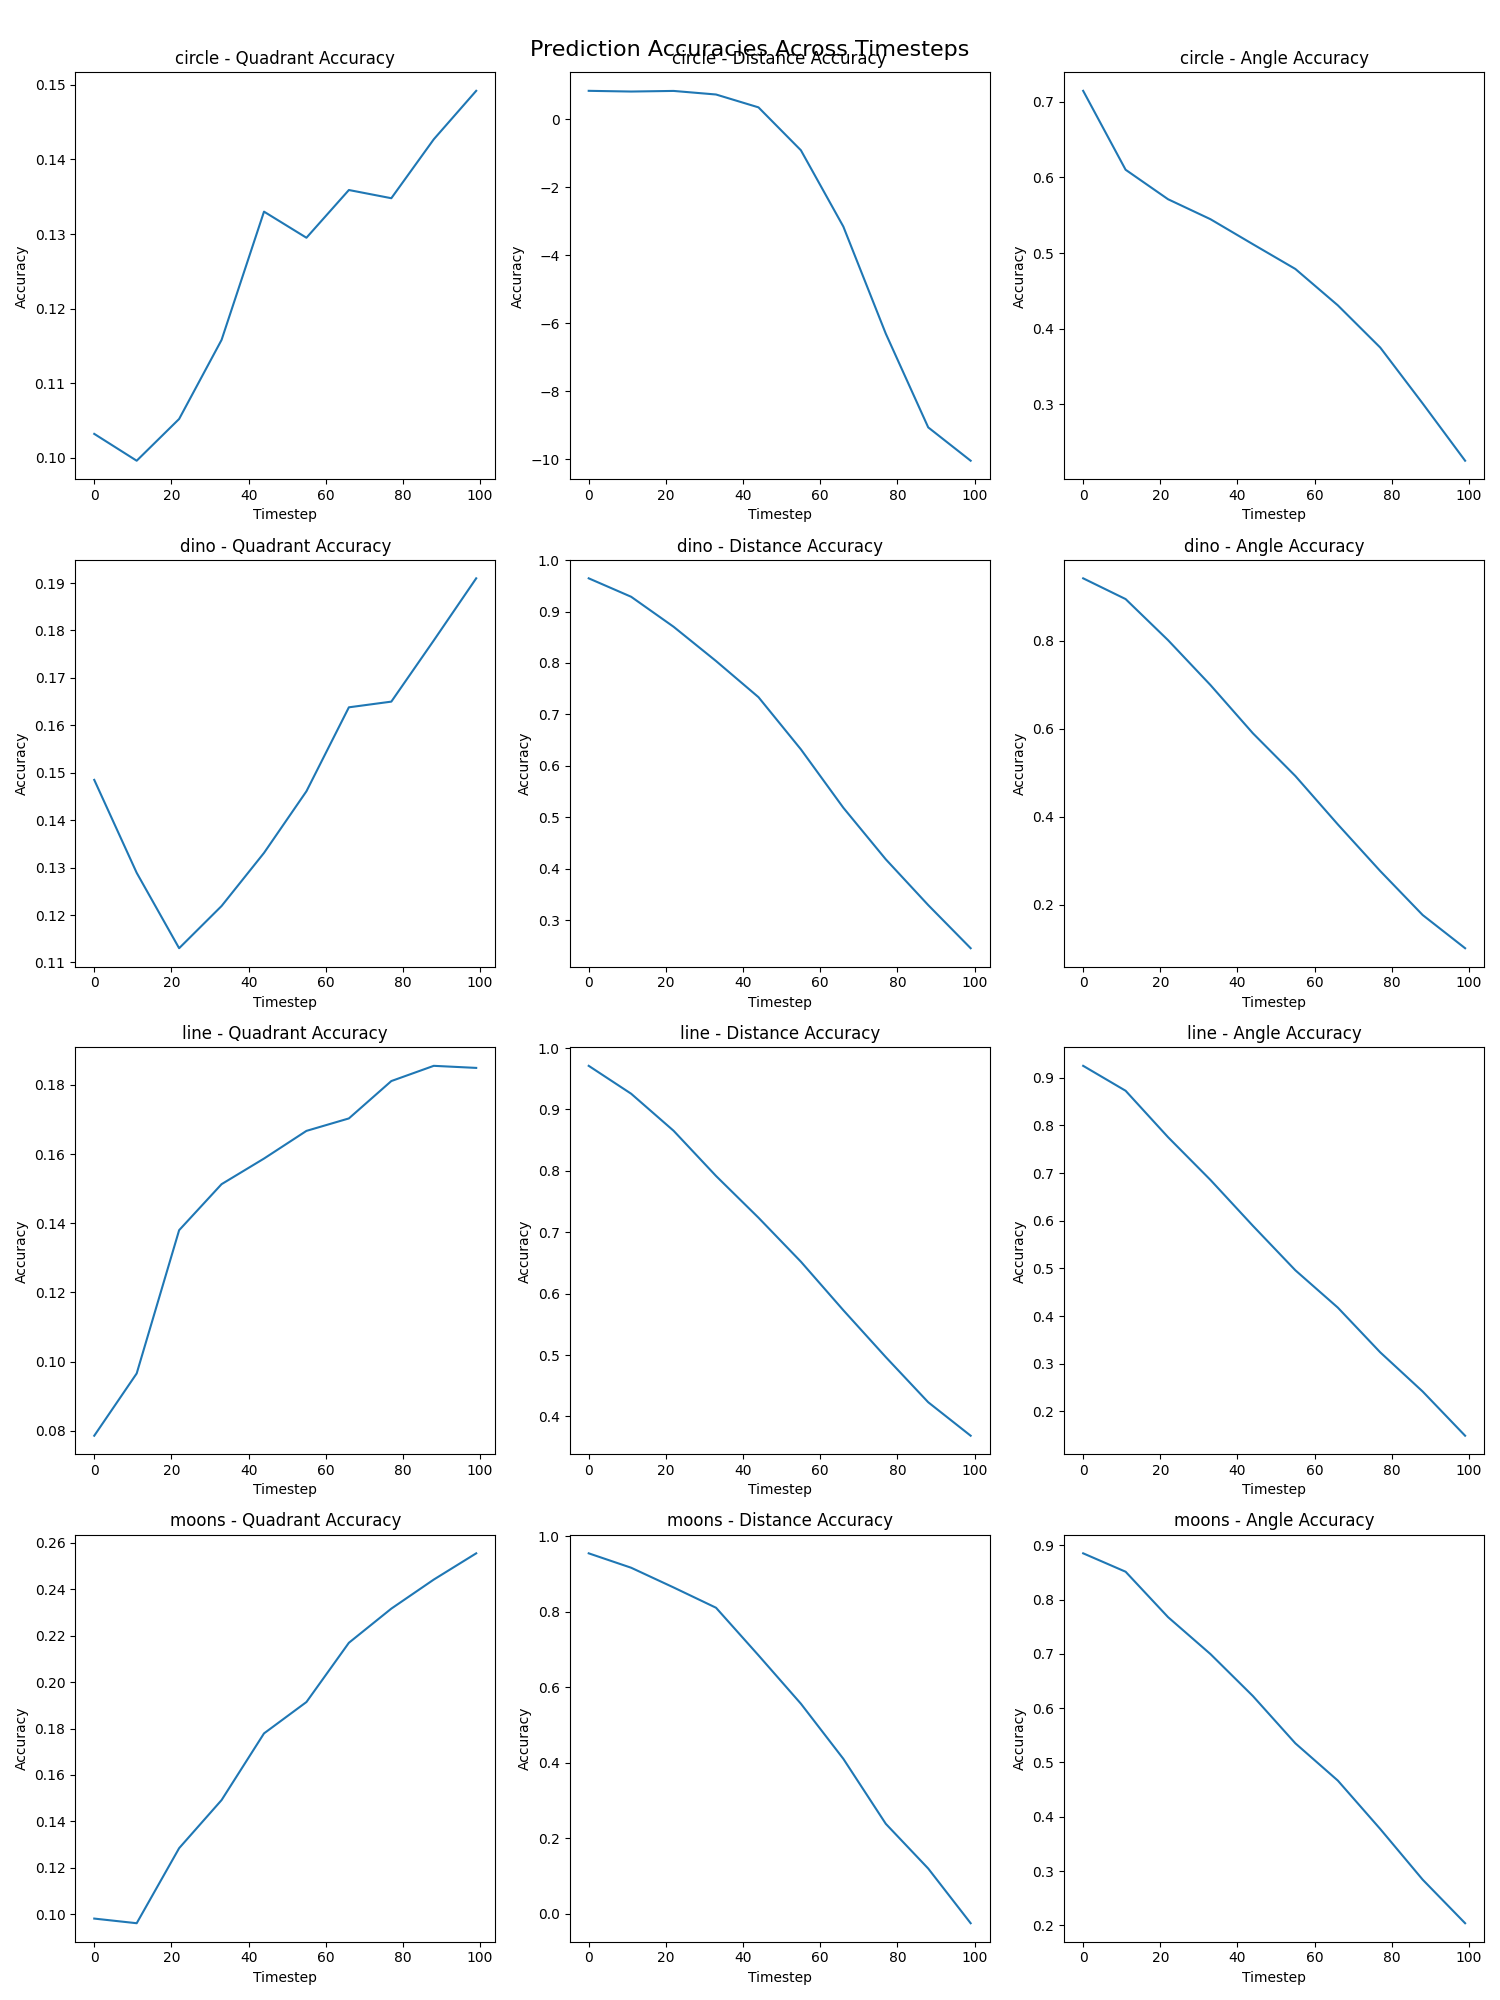
\includegraphics[width=\textwidth]{prediction_accuracies.png}
    \caption{Prediction accuracies for quadrant, distance, and angle across diffusion timesteps for different datasets.}
    \label{fig:prediction_accuracies}
\end{figure}

Additionally, we generate samples from the trained model to visually assess the quality of the learned distributions. Figure \ref{fig:generated_images} displays examples of the generated samples for each dataset, demonstrating the model's ability to capture the underlying distributions accurately.

\begin{figure}[t]
    \centering
    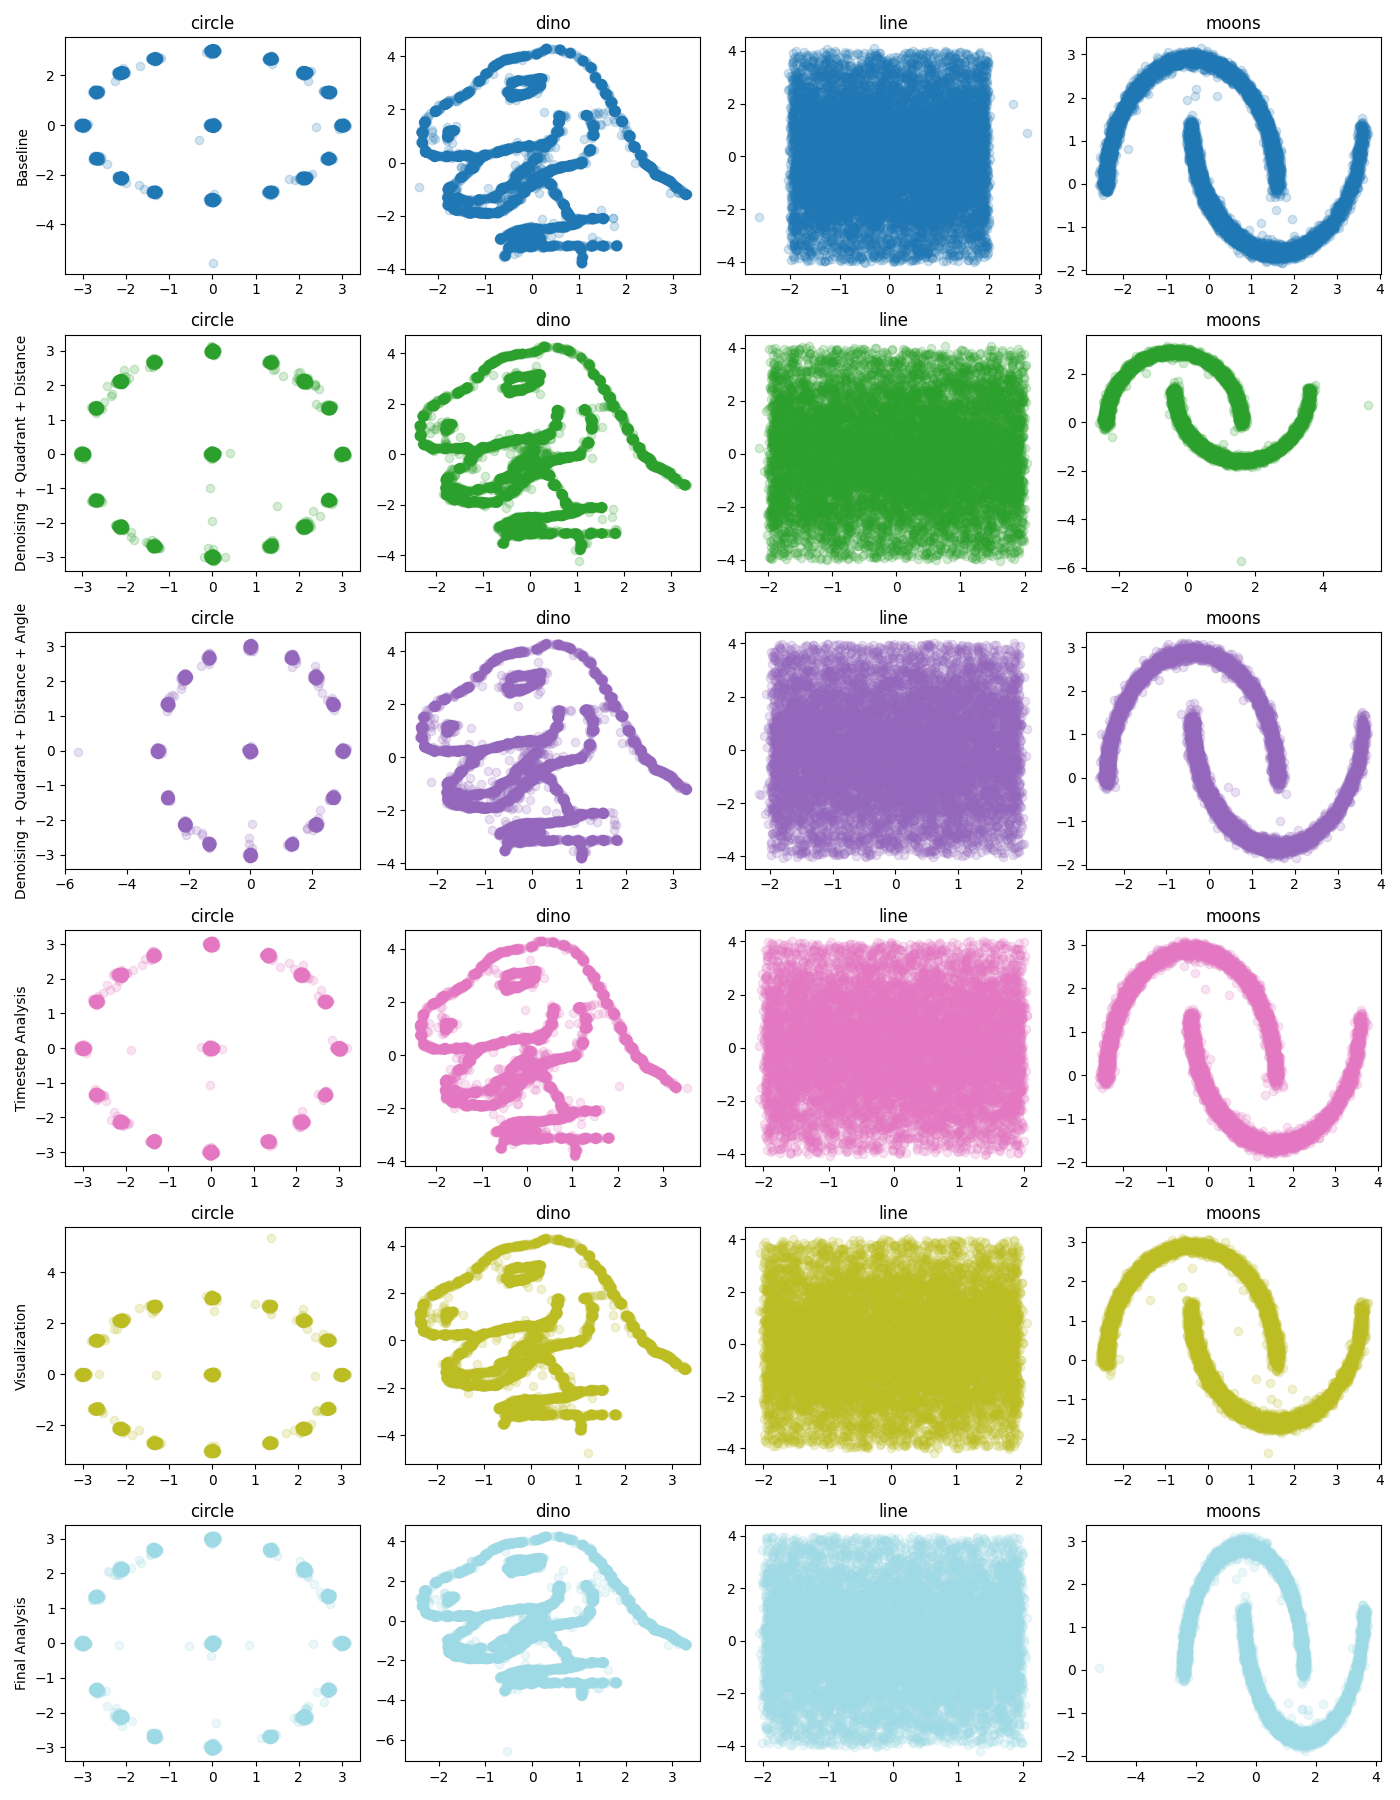
\includegraphics[width=\textwidth]{generated_images.png}
    \caption{Generated samples for circle, dino, line, and moons datasets.}
    \label{fig:generated_images}
\end{figure}

This comprehensive evaluation approach allows us to gain insights into how the model progressively learns to capture and reconstruct various aspects of the data distribution throughout the diffusion process. The results of our experiments are presented in Section \ref{sec:results}, including detailed analysis of the prediction accuracies and generated samples.

% EXAMPLE FIGURE: REPLACE AND ADD YOUR OWN FIGURES / CAPTIONS
\begin{figure}[t]
    \centering
    \begin{subfigure}{0.9\textwidth}
        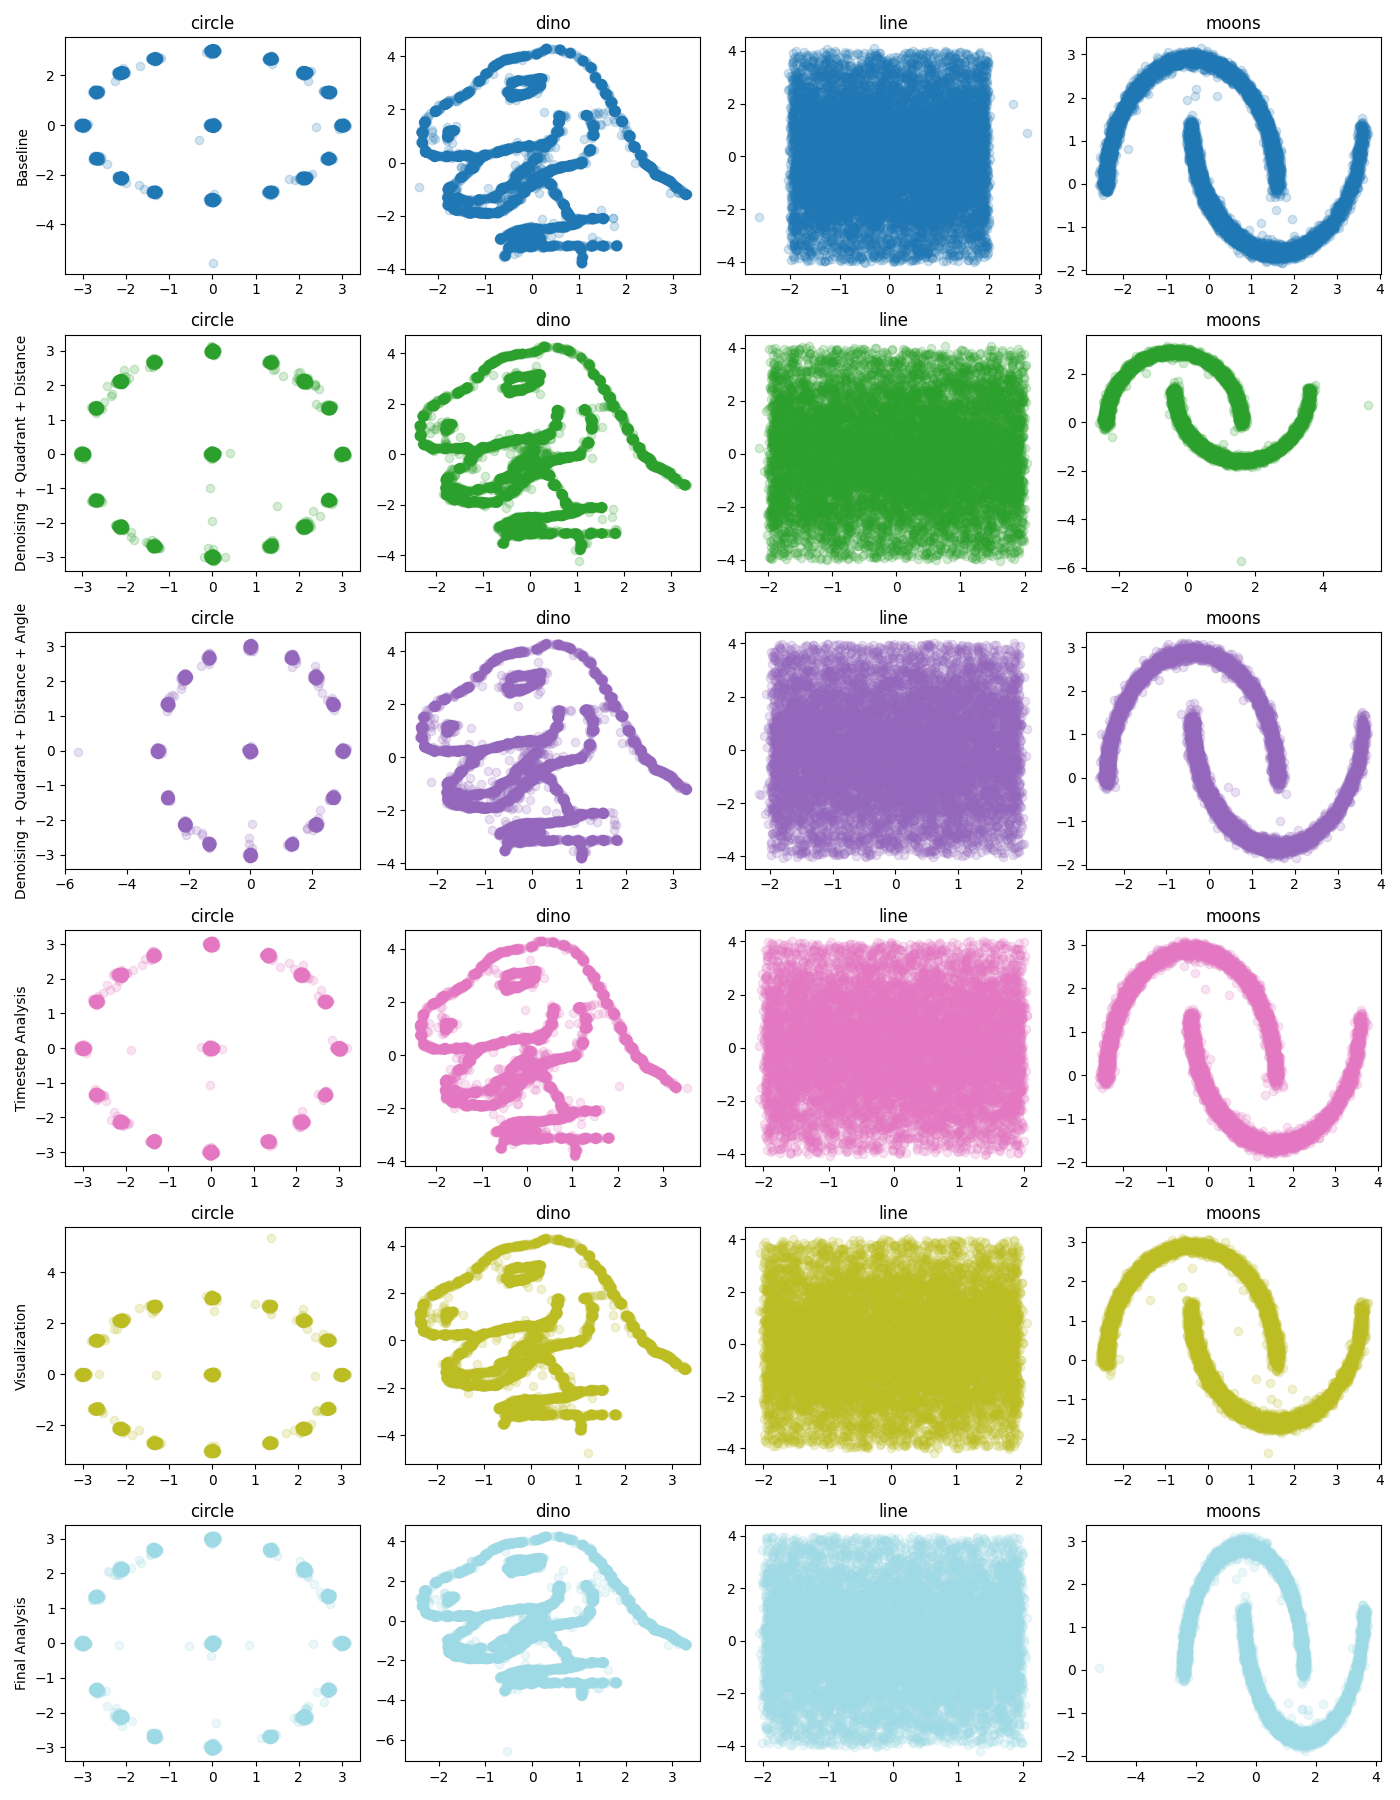
\includegraphics[width=\textwidth]{generated_images.png}
        \label{fig:diffusion-samples}
    \end{subfigure}
    \caption{PLEASE FILL IN CAPTION HERE}
    \label{fig:first_figure}
\end{figure}

\section{Results}
\label{sec:results}

Our experiments analyze the learning dynamics of diffusion models in low-dimensional spaces, focusing on how these models progressively understand and reconstruct data properties throughout the diffusion process. We present results from training our modified Denoising Diffusion Probabilistic Model (DDPM) on four distinct 2D datasets: circle, dino, line, and moons.

\subsection{Model Performance Across Datasets}

Table \ref{tab:model_performance} summarizes the key performance metrics for each dataset, including training time, evaluation loss components, inference time, and KL divergence between the generated and real data distributions.

\begin{table}[h]
\centering
\caption{Model performance across datasets}
\label{tab:model_performance}
\begin{tabular}{lcccc}
\toprule
Metric & Circle & Dino & Line & Moons \\
\midrule
Training Time (s) & 46.99 & 48.10 & 49.67 & 46.41 \\
Total Eval Loss & 0.5792 & 0.7751 & 0.9134 & 0.7011 \\
Denoising Loss & 0.4408 & 0.6626 & 0.8045 & 0.6115 \\
Quadrant Loss & 0.1930 & 0.2138 & 0.1918 & 0.1736 \\
Distance Loss & 0.0874 & 0.2392 & 0.2517 & 0.1873 \\
Angle Loss & 1.1034 & 0.6720 & 0.6454 & 0.5349 \\
Inference Time (s) & 0.1302 & 0.1285 & 0.1303 & 0.1187 \\
KL Divergence & 0.3560 & 1.4280 & 0.1679 & 0.0945 \\
\bottomrule
\end{tabular}
\end{table}

The model demonstrates consistent performance across datasets, with training times ranging from 46 to 50 seconds and inference times around 0.13 seconds for generating 10,000 samples. This efficiency is noteworthy given the model's ability to perform multiple prediction tasks simultaneously with the denoising process.

\subsection{Learning Dynamics and Prediction Accuracies}

Figure \ref{fig:prediction_accuracies} illustrates how the model's understanding of data properties evolves throughout the diffusion process. Key observations include:

\begin{itemize}
    \item Quadrant prediction accuracy improves rapidly in the early timesteps for all datasets, indicating quick learning of broad spatial regions.
    \item Distance prediction accuracy shows more gradual improvement, with better performance on circle and moons datasets compared to dino and line.
    \item Angle prediction accuracy varies most across datasets, with the circle dataset showing the most consistent improvement.
\end{itemize}

These observations suggest that the model learns different data properties at varying rates, depending on the underlying structure of the dataset.

\subsection{Quality of Generated Samples}

Figure \ref{fig:generated_images} demonstrates the model's ability to capture the underlying distributions accurately. The generated samples closely resemble the original datasets, with the circle and moons datasets showing particularly high fidelity. The dino dataset, being the most complex, shows some loss of fine details but maintains the overall structure. This visual assessment is supported by the KL divergence values in Table \ref{tab:model_performance}, which show lower divergence for simpler datasets (moons and line) and higher divergence for more complex ones (dino and circle).

\subsection{Limitations and Future Directions}

Despite the promising results, our approach has some limitations:

\begin{itemize}
    \item The model shows varying performance across datasets, with more complex structures (e.g., the dino dataset) presenting greater challenges.
    \item The angle prediction task consistently shows higher loss compared to other auxiliary tasks, suggesting that capturing angular information is more challenging for the model.
    \item Our experiments used fixed hyperparameters across all datasets, which may not be optimal for each individual dataset.
\end{itemize}

Future work could explore more complex datasets, alternative model architectures (particularly for improving angle prediction), dataset-specific hyperparameter tuning, additional auxiliary tasks, and extension to higher-dimensional data.

By addressing these areas, we can further elucidate the learning process of diffusion models and potentially improve their performance and interpretability in more complex, high-dimensional settings.

\section{Conclusions and Future Work}
\label{sec:conclusion}

In this paper, we presented a novel approach to analyzing the learning dynamics of diffusion models in low-dimensional spaces. By incorporating auxiliary prediction tasks into the diffusion process, we gained valuable insights into how these models progressively understand and reconstruct various aspects of data distributions.

Our key findings include:
\begin{itemize}
    \item The model quickly learns to distinguish broad spatial regions (quadrants) in early diffusion timesteps.
    \item More complex properties, such as distances and angles, are learned more gradually throughout the diffusion process.
    \item The model's performance varies across different dataset structures, with simpler geometries generally yielding better results.
    \item The approach is computationally efficient, maintaining consistent training and inference times across datasets while performing multiple prediction tasks.
\end{itemize}

These insights contribute to a deeper understanding of diffusion models' inner workings and pave the way for potential improvements in model architectures and training strategies.

Future research directions include:
\begin{itemize}
    \item Extending the approach to more complex, higher-dimensional datasets to test scalability and generalizability.
    \item Exploring alternative model architectures to address challenges in capturing certain data properties, particularly angular information.
    \item Investigating dataset-specific hyperparameter tuning to optimize performance across various data structures.
    \item Developing additional auxiliary tasks to provide even more granular insights into the learning process.
    \item Applying the insights gained from this study to improve the interpretability and performance of diffusion models in practical applications.
\end{itemize}

By pursuing these avenues, we aim to further advance our understanding of diffusion models and enhance their capabilities in generating high-quality samples across a wide range of domains.

\bibliographystyle{iclr2024_conference}
\bibliography{references}

\end{document}
